%%%%%%%%%%%%%%%%%%%%%%%%%%%%%%%%%%%%%%%%%%%%%%%%%%%%%%%%%%%%%%%%%%%%
%%%%% DOC ARCHITECTURE : MAIN %%%%%
%%%%%%%%%%%%%%%%%%%%%%%%%%%%%%%%%%%%%%%%%%%%%%%%%%%%%%%%%%%%%%%%%%%%


\documentclass[a4paper]{article}


%%%%% Packages %%%%%

%%%%% Langage %%%%%
\usepackage[frenchb]{babel}
\usepackage[utf8]{inputenc}
\usepackage[T1]{fontenc}
%%%%% Graphique %%%%%
\usepackage{graphicx}
\usepackage{wrapfig}
%%%%% Mise en page %%%%%
\usepackage{hyperref}
\usepackage{fancyhdr}
\usepackage{colortbl}
\usepackage{titlesec}



%%%%% Macros %%%%
%%%%%%%%%%%%%%%%%%%%%%%%%%%%%%%%%%%%%%%%%%%%%%%%%%%%%%%%%%%%%%%%%%%%
%%%%% MACROS %%%%%
%%%%%%%%%%%%%%%%%%%%%%%%%%%%%%%%%%%%%%%%%%%%%%%%%%%%%%%%%%%%%%%%%%%%

%%%%% Ligne de séparation %%%%%
\newcommand{\HRule}{\rule{\linewidth}{0.5mm}}

%%%%% Recoloration des liens %%%%%
\hypersetup{	colorlinks = true,
			breaklinks = true,
     		linkcolor = {blue},
     		urlcolor = {blue},}

%%%%% Création de nouvelles couleurs %%%%%
\definecolor{lightgray}{rgb}{0.75,0.75,0.75}

%%%%% Saut de ligne %%%%%
\newcommand{\NewLine}{\vspace{0.5cm}}

%%%%% Inclusion d'en-tête %%%%%
\pagestyle{fancy}
\setlength{\headheight}{23pt}	% Correction du warning \headheight is too small
\lhead{Armor Editor}
\rhead{Documentation développeur}


%%%%%%%%%%%%%%%%%%%%%%%%%%%%%%%%%%%%%%%%%%%%%%%%%%%%%%%%%%%%%%%%%%%%
%%%%% DOCUMENT %%%%%
%%%%%%%%%%%%%%%%%%%%%%%%%%%%%%%%%%%%%%%%%%%%%%%%%%%%%%%%%%%%%%%%%%%%

\begin{document}

%%%%% Page de garde %%%%%
%%%%%%%%%%%%%%%%%%%%%%%%%%%%%%%%%%%%%%%%%%%%%%%%%%%%%%%%%%%%%%%%%%%%
%%%%% PAGE DE GARDE %%%%%
%%%%%%%%%%%%%%%%%%%%%%%%%%%%%%%%%%%%%%%%%%%%%%%%%%%%%%%%%%%%%%%%%%%%

\begin{titlepage}
\begin{center}

%%% Logo et sous-titre

\includegraphics[width=0.45\textwidth]{../figures/logoUN.png}~\\[2cm]

\LARGE{Master 1 \textsc{Alma}}\\[1.5cm]

\Large{Projet de Conception de Logiciels Extensibles}\\[0.5cm]

%%% Titre
\HRule \\[0.4cm]
{ \huge \bfseries Documentation Développeur \\[0.4cm] }
\HRule \\[1.5cm]

%%% Auteurs et professeur
\normalsize	
\emph{\'Etudiants :}\\
Coraline \textsc{Marie}, Vincent \textsc{Raveneau} et Quentin \textsc{Moriceau}

\vspace{0.5cm}

\emph{Encadrant :} \\
Gilles \textsc{Ardourel}

\vfill

%%% Date de rendu
{\large 30 mars 2014}

\end{center}
\end{titlepage}



%%%%% Cahier des charges %%%%%
\section{Cahier des charges}

Dans le cadre du cours de \textit{Conception de logiciels extensibles}, les étudiants du Master 1 \textsc{Alma} avaient pour objectif de concevoir un logiciel extensible, ainsi que quelques plugins agissant sur des données quelconques. Les fonctionnalités du logiciel ainsi que celles des plugins étaient libres de choix, cependant il fallait qu'elles permettent de créer, d'afficher et de modifier des données.\\

Ce rapport a donc été écrit dans le but d'expliquer comment notre groupe de travail s'est organisé pour la conception du projet \textsc{\'Editeur d'Armure}. Il présente les différentes étapes de notre travail, depuis l'imagination, jusqu'à la réalisation de notre projet, mais aussi la répartitions des tâches entre les étudiants.



%%%%% Organisation du projet %%%%%
\section{Organisation du projet}

Ce projet s'est étalé sur environ 3 mois de programmation. Pour se faire, le travail a été divisé en plusieurs parties :
\begin{itemize}
	\item la conception du projet;
	\item la création de la base ArmorEditor;
	\item la mise en place du pluginManager;
	\item la production des premiers plugins : \texttt{CreationArmure} et \texttt{AffichageConsole};
	\item la mise en place du plugin pour l'interface graphique : \texttt{AffichageGraphique};
	\item la création d'autres plugins de manipulation de données : \texttt{ModificationArmure} et \texttt{CreationArmureFichier};
	\item le refactoring;
\end{itemize}
\vspace{0.5cm}

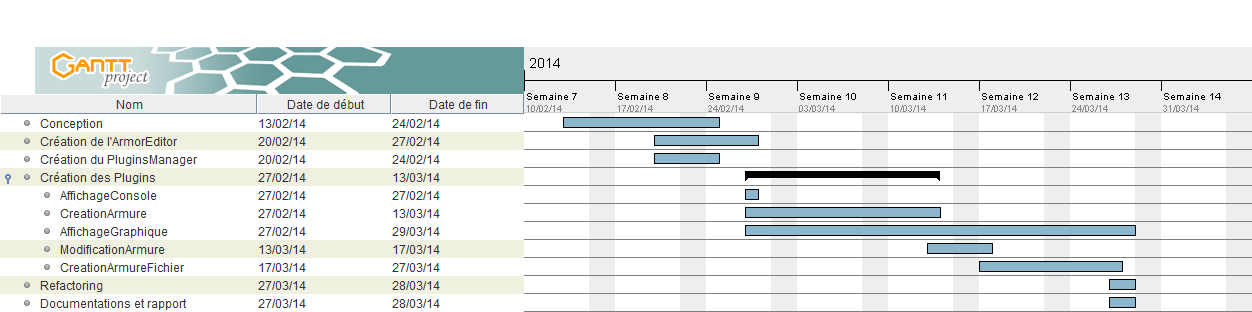
\includegraphics[width=\textwidth]{../figures/gantt.png}\\

Le diagramme de Gantt ci-dessus représente les différentes étapes de notre travail.\\

Pour que la programmation soit optimisée, chaque étudiant s'est spécialisé dans une partie du code :
\begin{itemize}
	\item Quentin : plugin d'affichage graphique;
	\item Coraline : plugins d'affichages et de manipulations des données;  
	\item Vincent : coeur de l'application (pluginManager, fichiers de configuration, \dots) et corrections des différentes parties du projet.
\end{itemize}


\end{document}
